% Requires:
% \usepackage{pgfplots}
% \pgfplotsset{compat=1.18}
% \usepackage{subcaption}

\section*{Current Experiment Charts}

\subsection*{1. Arxiv Inference Result Comparison}

\begin{figure}[htbp]
\centering
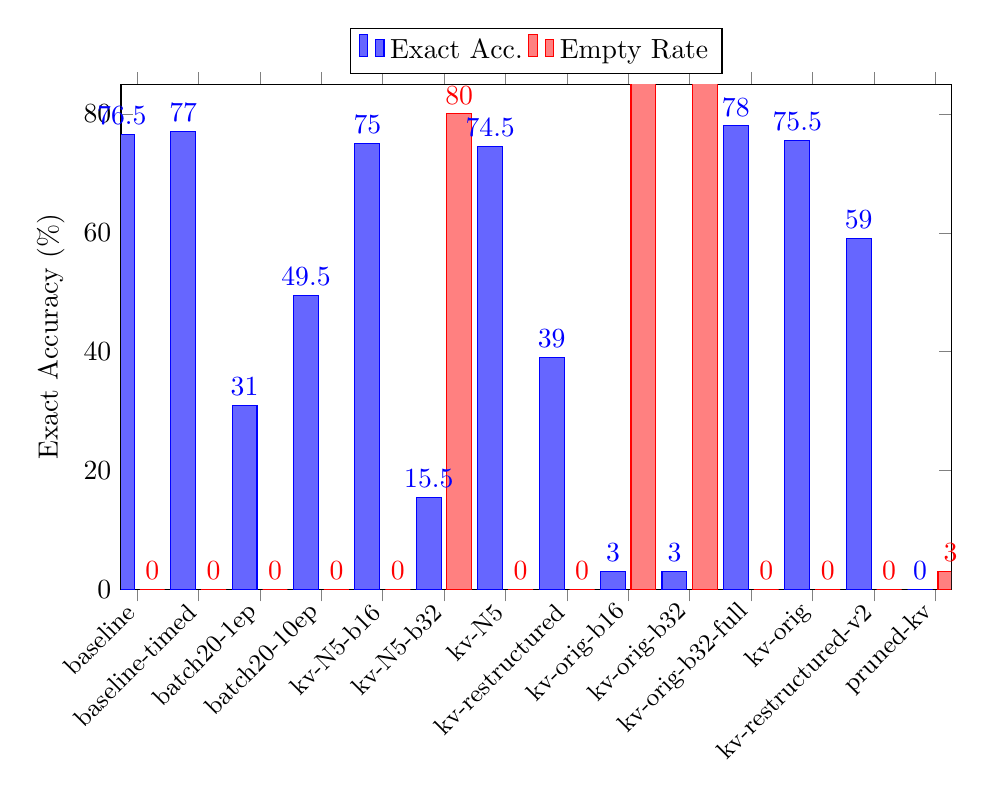
\begin{tikzpicture}
\begin{axis}[
    width=\textwidth,
    height=8cm,
    ybar,
    bar width=9pt,
    ymin=0,
    ymax=85,
    ylabel={Exact Accuracy (\%)},
    symbolic x coords={
        baseline,
        baseline-timed,
        batch20-1ep,
        batch20-10ep,
        kv-N5-b16,
        kv-N5-b32,
        kv-N5,
        kv-restructured,
        kv-orig-b16,
        kv-orig-b32,
        kv-orig-b32-full,
        kv-orig,
        kv-restructured-v2,
        pruned-kv
    },
    xtick=data,
    x tick label style={rotate=45,anchor=east,font=\small},
    nodes near coords,
    nodes near coords align={vertical},
    enlarge x limits=0.02,
    legend style={at={(0.5,1.02)},anchor=south,legend columns=3},
]
\addplot+[fill=blue!60] coordinates {
    (baseline,76.50)
    (baseline-timed,77.00)
    (batch20-1ep,31.00)
    (batch20-10ep,49.50)
    (kv-N5-b16,75.00)
    (kv-N5-b32,15.50)
    (kv-N5,74.50)
    (kv-restructured,39.00)
    (kv-orig-b16,3.00)
    (kv-orig-b32,3.00)
    (kv-orig-b32-full,78.00)
    (kv-orig,75.50)
    (kv-restructured-v2,59.00)
    (pruned-kv,0.00)
};
\addlegendentry{Exact Acc.}

\addplot+[fill=red!50] coordinates {
    (baseline,0.00)
    (baseline-timed,0.00)
    (batch20-1ep,0.00)
    (batch20-10ep,0.00)
    (kv-N5-b16,0.00)
    (kv-N5-b32,80.00)
    (kv-N5,0.00)
    (kv-restructured,0.00)
    (kv-orig-b16,96.00)
    (kv-orig-b32,96.00)
    (kv-orig-b32-full,0.00)
    (kv-orig,0.00)
    (kv-restructured-v2,0.00)
    (pruned-kv,3.00)
};
\addlegendentry{Empty Rate}
\end{axis}
\end{tikzpicture}
\caption{Comparison of exact accuracy and empty-output rate across existing \texttt{results/*.jsonl} files on arxiv NC.}
\end{figure}

\subsection*{2. MoE Hot-Swap Batch Sweep}

\begin{figure}[htbp]
\centering
\begin{subfigure}{0.49\textwidth}
\centering
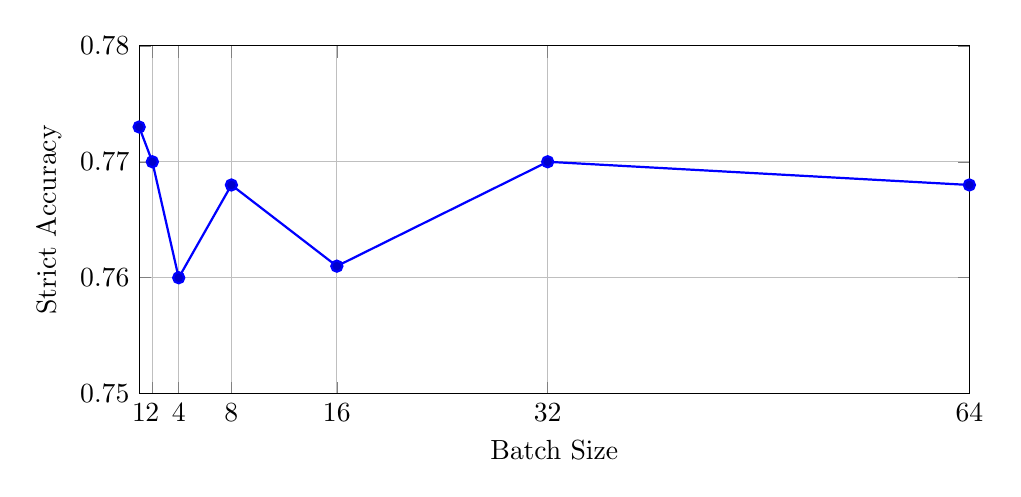
\begin{tikzpicture}
\begin{axis}[
    width=\textwidth,
    height=6cm,
    xlabel={Batch Size},
    ylabel={Strict Accuracy},
    xmin=1, xmax=64,
    ymin=0.75, ymax=0.78,
    xtick={1,2,4,8,16,32,64},
    grid=major,
    mark=*,
]
\addplot+[blue, thick] coordinates {
    (1,0.7730)
    (2,0.7700)
    (4,0.7600)
    (8,0.7680)
    (16,0.7610)
    (32,0.7700)
    (64,0.7680)
};
\end{axis}
\end{tikzpicture}
\caption{Strict accuracy vs. batch size}
\end{subfigure}
\hfill
\begin{subfigure}{0.49\textwidth}
\centering
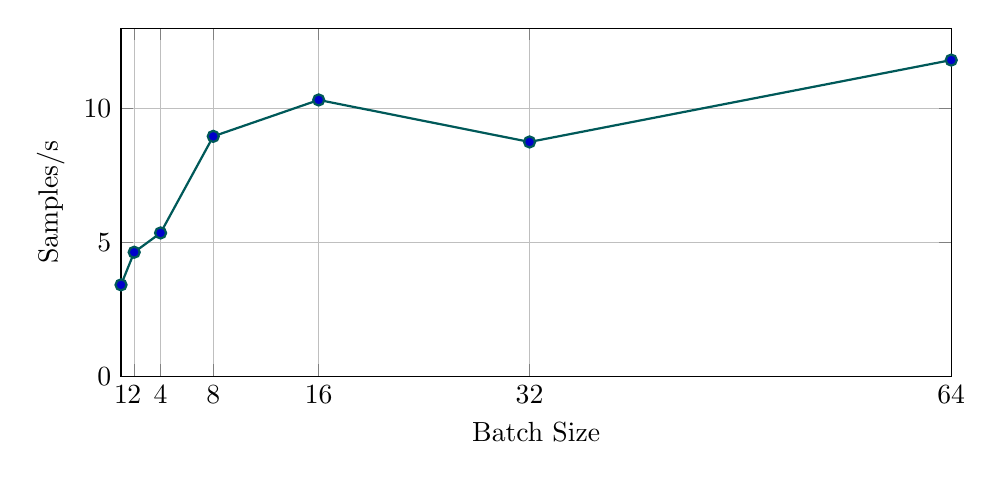
\begin{tikzpicture}
\begin{axis}[
    width=\textwidth,
    height=6cm,
    xlabel={Batch Size},
    ylabel={Samples/s},
    xmin=1, xmax=64,
    ymin=0, ymax=13,
    xtick={1,2,4,8,16,32,64},
    grid=major,
    mark=square*,
]
\addplot+[teal!70!black, thick] coordinates {
    (1,3.41)
    (2,4.63)
    (4,5.35)
    (8,8.96)
    (16,10.32)
    (32,8.75)
    (64,11.81)
};
\end{axis}
\end{tikzpicture}
\caption{Throughput vs. batch size}
\end{subfigure}
\caption{MoE hot-swap evaluation sweep on 1000 arxiv NC samples. Accuracy is stable across \texttt{bs=1..64}, while throughput peaks at \texttt{bs=64}.}
\end{figure}

\subsection*{3. Quantization Comparison on Cora NC}

\begin{figure}[htbp]
\centering
\begin{subfigure}{0.49\textwidth}
\centering
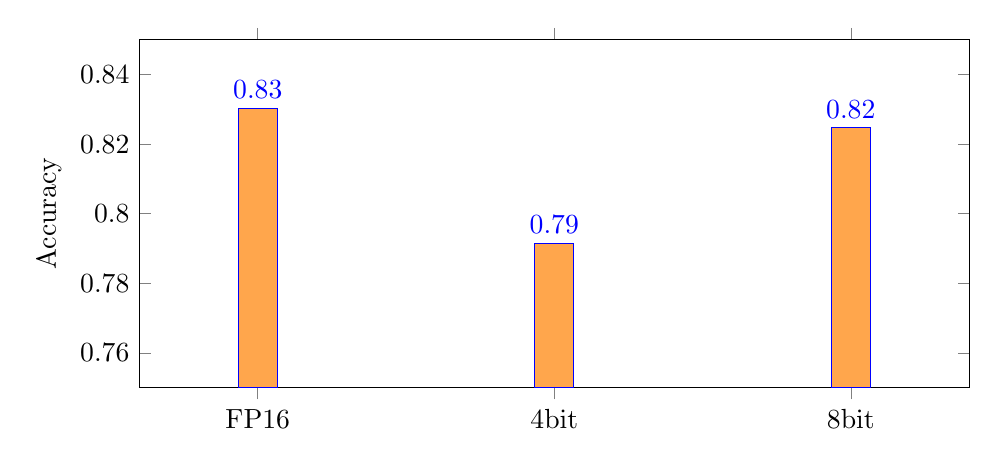
\begin{tikzpicture}
\begin{axis}[
    width=\textwidth,
    height=6cm,
    ybar,
    bar width=14pt,
    ymin=0.75,
    ymax=0.85,
    ylabel={Accuracy},
    symbolic x coords={FP16,4bit,8bit},
    xtick=data,
    nodes near coords,
    enlarge x limits=0.2,
]
\addplot+[fill=orange!70] coordinates {
    (FP16,0.8303)
    (4bit,0.7915)
    (8bit,0.8247)
};
\end{axis}
\end{tikzpicture}
\caption{Quantization accuracy}
\end{subfigure}
\hfill
\begin{subfigure}{0.49\textwidth}
\centering
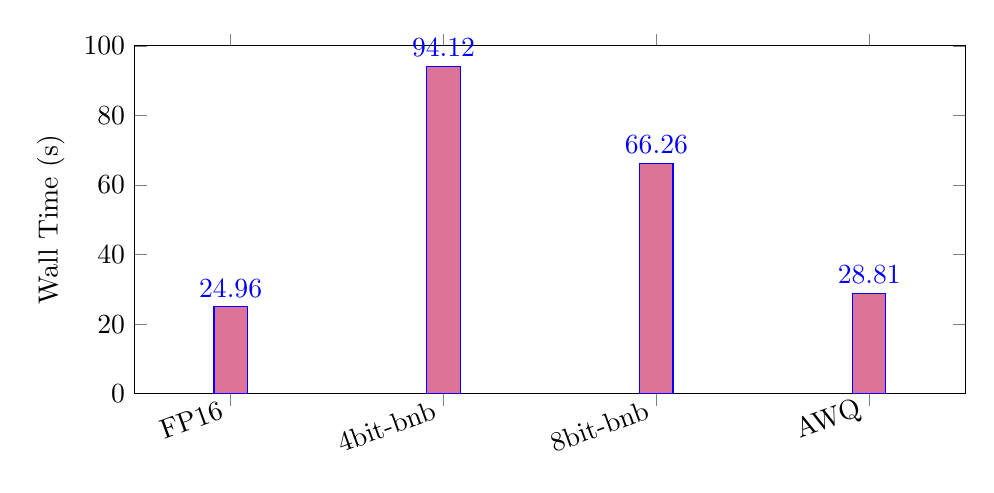
\begin{tikzpicture}
\begin{axis}[
    width=\textwidth,
    height=6cm,
    ybar,
    bar width=12pt,
    ymin=0,
    ymax=100,
    ylabel={Wall Time (s)},
    symbolic x coords={FP16,4bit-bnb,8bit-bnb,AWQ},
    xtick=data,
    x tick label style={rotate=20,anchor=east},
    nodes near coords,
    enlarge x limits=0.15,
]
\addplot+[fill=purple!55] coordinates {
    (FP16,24.96)
    (4bit-bnb,94.12)
    (8bit-bnb,66.26)
    (AWQ,28.81)
};
\end{axis}
\end{tikzpicture}
\caption{End-to-end wall time}
\end{subfigure}
\caption{Quantization results on cora NC. FP16 has the best accuracy, while AWQ is close to FP16 in speed with much lower memory usage according to the benchmark table.}
\end{figure}

\subsection*{4. Optional: Training Loss Snapshot}

\begin{figure}[htbp]
\centering
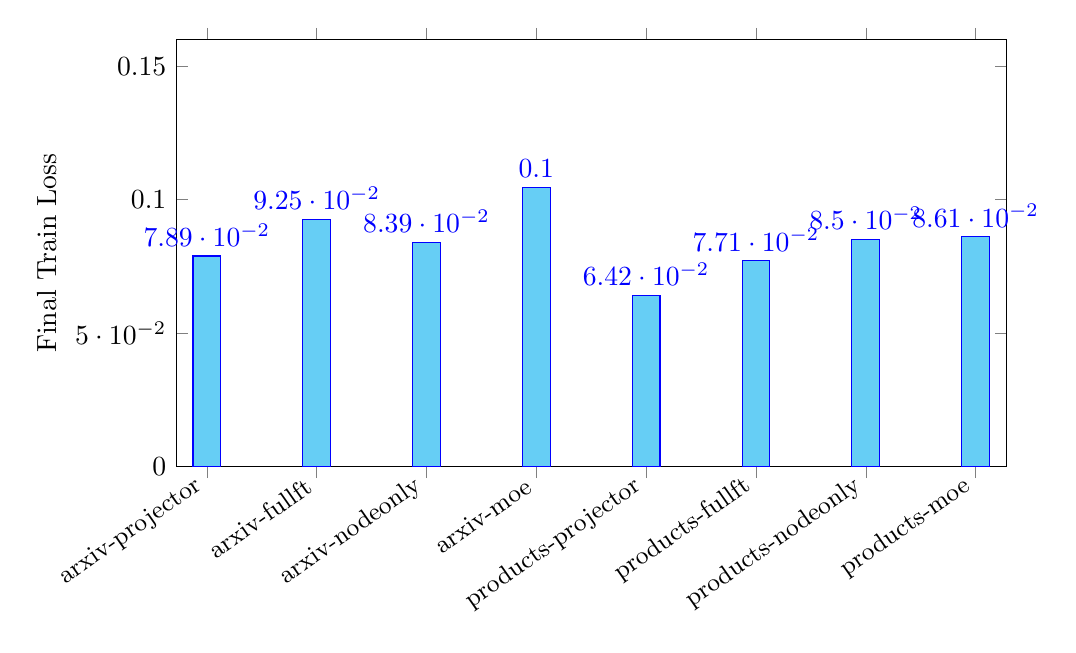
\begin{tikzpicture}
\begin{axis}[
    width=\textwidth,
    height=7cm,
    ybar,
    bar width=10pt,
    ymin=0,
    ymax=0.16,
    ylabel={Final Train Loss},
    symbolic x coords={
        arxiv-projector,
        arxiv-fullft,
        arxiv-nodeonly,
        arxiv-moe,
        products-projector,
        products-fullft,
        products-nodeonly,
        products-moe
    },
    xtick=data,
    x tick label style={rotate=35,anchor=east,font=\small},
    nodes near coords,
    enlarge x limits=0.04,
]
\addplot+[fill=cyan!60] coordinates {
    (arxiv-projector,0.0789)
    (arxiv-fullft,0.0925)
    (arxiv-nodeonly,0.0839)
    (arxiv-moe,0.1046)
    (products-projector,0.0642)
    (products-fullft,0.0771)
    (products-nodeonly,0.0850)
    (products-moe,0.0861)
};
\end{axis}
\end{tikzpicture}
\caption{Final training loss snapshot for major arxiv/products NC runs with available W\&B summaries.}
\end{figure}

